\documentclass[runningheads,a4paper]{llncs}

\usepackage[cp1250]{inputenc}  % or [cp1250], or [latin2], or whatever
                               % suitable for your system
\usepackage{amssymb}
\setcounter{tocdepth}{3}
\usepackage{graphicx}

\usepackage{url}

\newcommand{\keywords}[1]{\par\addvspace\baselineskip
\noindent\keywordname\enspace\ignorespaces#1}


\begin{document}

\mainmatter  % start of an individual contribution

\title{Repository, Framework and Methods for Semantic Annotation}


\author{Jan Dedek \and Peter Vojtas}

\institute{Charles University, Department of software engineering, Prague, Czech Republic \email{\{dedek, vojtas\}@ksi.mff.cuni.cz}
\and Academy of Sciences of the Czech Republic, Institute of Computer Science}

\maketitle


\begin{abstract}
.... Web Semantization is a concept we introduce in this paper. We understand Web Semantization as an automated process of increasing degree of semantic content on the web. Part of content of the web is further usable, semantic content (usually annotated) is more suitable for machine processing ....
\keywords{Web Content Mining, Web Content Machine Processing, Annotation, Linguistic Analysis}
\end{abstract}

\section{Introduction}
In their Scientific American 2001 article \cite{biblio:2001-Berners-Lee-SemanticWeb}, Tim Berners-Lee, James Hendler and Ora Lassila unveiled a nascent vision of the semantic web: a highly interconnected network of data that could be easily accessed and understood by a desktop or handheld machine. They painted a future of intelligent software agents that would ``answer to a particular question without our having to search for information or pore through results'' (quoted from \cite{biblio:feigenbaum_semantic_2007}). Lee Feigenbaum, Ivan Herman, Tonya Hongsermeier, Eric Neumann and Susie Stephens in their Scientific American 2007 article \cite{biblio:feigenbaum_semantic_2007} conclude that ``Grand visions rarely progress exactly as planned, but the Semantic Web is indeed emerging and is making online information more useful as ever''. L. Feigenbaum et al. support their claim with success of semantic web technology in drug discovery and health care (and several further applications). These are mainly corporate applications with data annotated by humans. Ben Adida when bridging clickable and Semantic Web with RDFa (\cite{biblio:AdidaClickable}) assumes also human (assisted) activity by annotations of newly created web resources. \par

........

Our web crawler (see Fig.\ref{img:Semantization}) downloads a part of the web to the web repository (Web Store). Resources with semantic content can be uploaded directly to the semantic repository (Semantic Store). Extractor~1 (classifier) extracts those parts of Web Store which are suitable for further semantic enrichment (we are able to enrich only a part of resources). More semantic content is created by several extractors and annotators in several phases. The emphasis of this paper is on the automation and the usage of such extracted/enriched data.

\begin{figure}
\centering
\includegraphics[height=.8\hsize, width=\hsize]{img/Semantization}
\caption{The process of semantization of the Web}
\label{img:Semantization}
\end{figure}



\section{Obr�zky}


\begin{figure}
\centerline{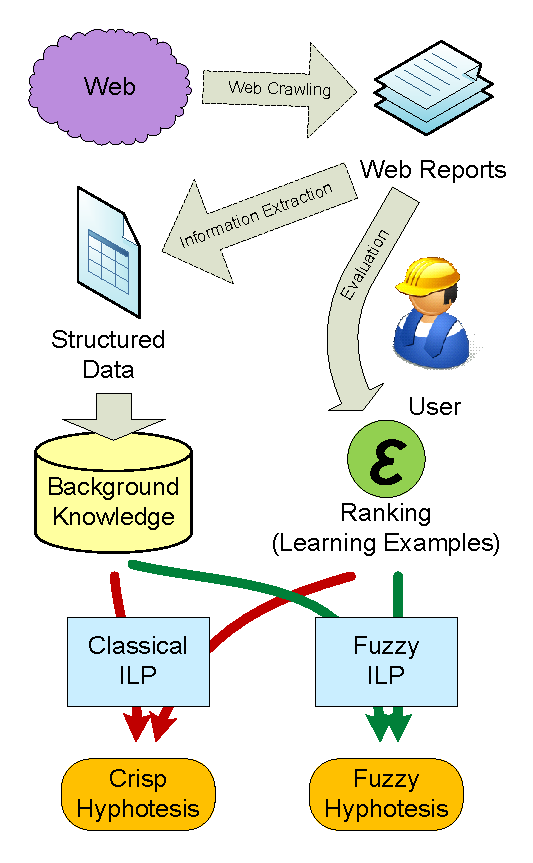
\includegraphics[width=.5\hsize]{img/schema}}
\caption{Schema of presented work (text part).}
\label{img:schema}
\end{figure}


\begin{figure}
\centerline{\includegraphics[width=.7\hsize]{img/message}}
\caption{Example of analyzed web report.}
\label{img:message}
\end{figure}


\begin{figure}
\centerline{\framebox{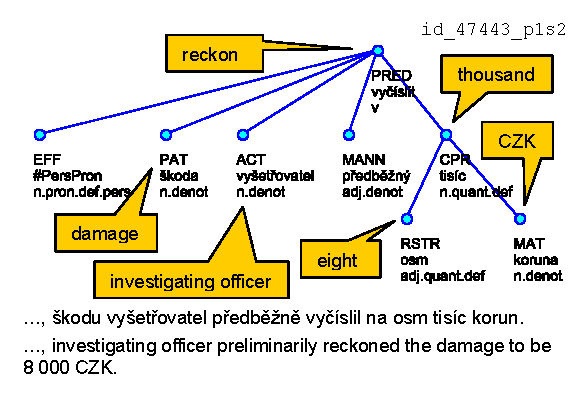
\includegraphics[width=.7\hsize]{img/tree}}}
\caption{Example of linguistic tree of one of analyzed sentences.}
\label{img:tree}
\end{figure}


\begin{figure}
\centerline{\includegraphics[width=.7\hsize]{img/ranking_histogram}}
\caption{Frequency histogram of accident ranking.}
\label{img:ranking_histogram}
\end{figure}


\begin{figure}
\centerline{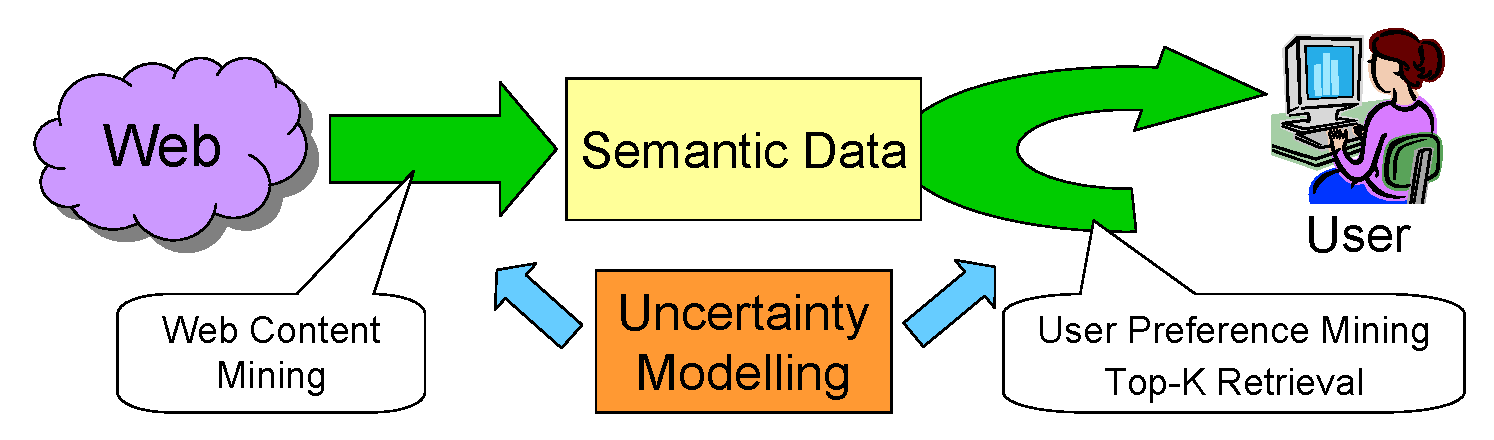
\includegraphics[width=.7\hsize]{img/Web2User}}
\caption{SemWeb 1ET100300419}
\label{img:uncert}
\end{figure}

\begin{figure}
\centerline{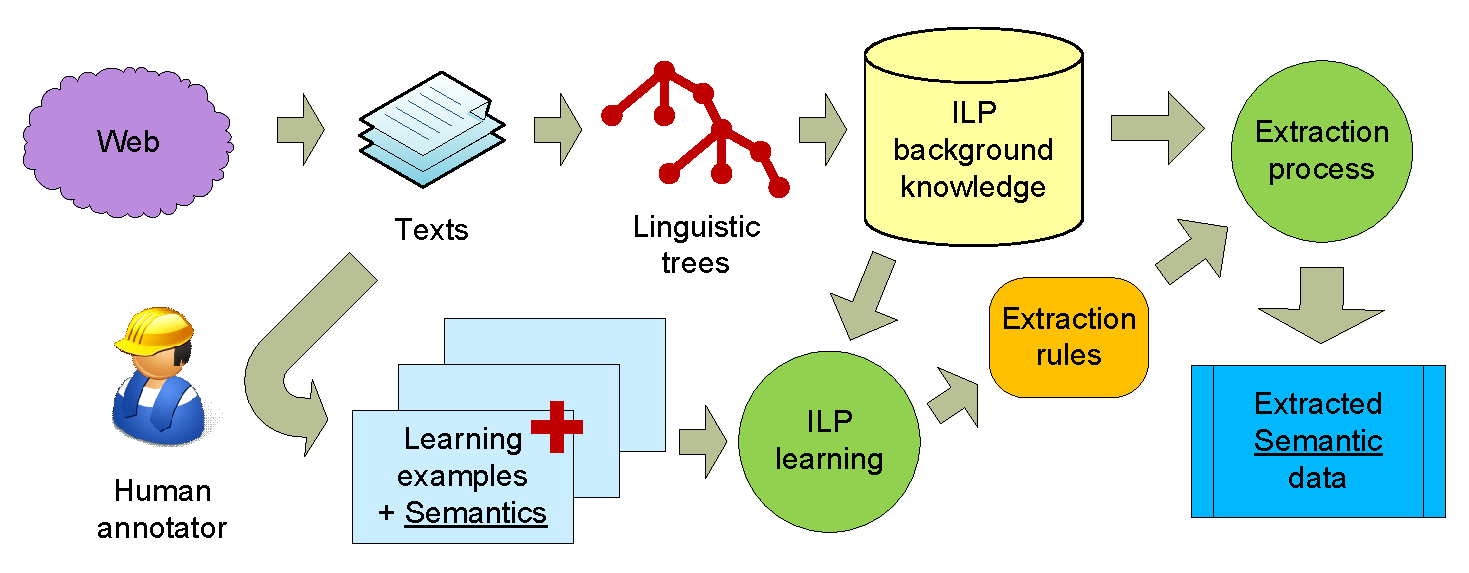
\includegraphics[width=\hsize]{img/DedVoj_ILP}}
\caption{Sch�ma z prentace ILP v Praze, \textbf{nepublikov�no}}
\label{img:schema_ILP}
\end{figure}



\section{Idea of Web semantization}

\begin{figure}
\label{fig:similarity}
\begin{center}
\begin{tabular}{|p{100pt}||p{100pt}|p{100pt}|} \hline
Type of annotation&Tabular pages&Textual pages\\ \hline\hline
Intermediate general&Uses similarities&Does not use similarities\\ \hline
Domain dependent&Does not use similarities&Uses similarities\\ \hline
\end{tabular}	
\end{center}
\caption{Use of similarity in annotation approaches}
\end{figure} 


Third important idea is to \textbf{design semantic repository}. It should store all the semantic data extracted by extraction tools and accessed thorough a semantic search engine. Of course many different problems (e.g. querying and scalability) are connected with this but they are at least partially solved now days. Let us mention work of our colleges \cite{biblio:DoTySemanticWeb2007} that is available for use.

The semantic repository should also contain some sort of uncertainty annotation besides above mentioned ontologies. The main reason is that annotation process is error prone and we can have in future different alternative annotation tools and aggregate results. This aspect is not further described in the paper but can be found with many details in \cite{biblio:DeEcDiscussionUncertainty2008} and \cite{biblio:EcHoUncertaintyIssues2008}.\par

Last, but also important idea is \textbf{(4) to design at least one agent} which will give evidence that our semantization really improved general web search. Besides using annotated data it should also contain some user dependent preference search capabilities.


\subsection{Extraction based on structural similarity}
First approach for domain independent intermediate information extraction and semantic annotation is to use the structural similarity in web pages containing large number of table cells and for each cell a link to detailed pages. This is often presented in web shops and on pages that presents more than one object (product offer). Each object is presented in a similar way and this fact can be exploited.

As web pages of web shops are intended for human usage creators have to make their comprehension easier. Acquaintance with several years of web shops has converged to a more or less similar design fashion. There are often cumulative pages with many products in a form of a table with cells and some brief description and then there are links detailed pages to each product.

There exist many extraction tools that can process web pages like this. Most complete recent survey can be found in \cite{biblio:Chang2006} and also in \cite{biblio:WebDataMining}.  We come with similar but also different solution divided into domain dependent and domain independent phases. See below for details.

\begin{figure}
\centering
\includegraphics[width=.6\hsize]{img/StructuralSimilarity}
\caption{Structural similarity in web pages}
\label{img:StructuralSimilarity}
\end{figure}

Our main idea (illustrated in the Figure \ref{img:StructuralSimilarity}) is to use a DOM tree representation of the summary web page and by breadth first search encounter similar subtrees. The similarity of these subtrees is used to determine the data region - a place where all the objects are stored. It is represented as a node in the DOM tree, underneath it there are the similar sub-trees, which are called data records.

Our ontology engineering part is based on a bottom-up approach of building ontologies. The first classes are `tabular page', `data region' and `data record' which are connected with properties `hasDataRegion' and `hasDataRecord'. Also, between data record and its detail \emph{Data\_region} and \emph{Detailed\_page} we have property `hasDetailPage'. Note that these concepts and properties have soft computing nature which can be modeled by a fuzzy ontology. For instance, being an instance has a degree of membership depending on the precision of our algorithm (dependent on similarity measures used to detect data regions and/or records). Using some heuristics we can detect what are resources described in this page (Tabular\_page describes rdfs:Resources). To detect possible attributes and even their values we explore similarities between data record content and corresponding detailed page content. The main idea is to find same pieces of text in the data record and in the detail page. This occurs often, because a brief summary of the object is present in the data record. Somewhere near the attribute values are located the names of attributes in the detail page. These names of attributes can be extracted. The extraction of attribute names is easy because on every detail page the names will be the same.  The names of attributes can be used in our low-level ontology as names of properties - each object will be represented by the URL of the detail page, and a set of properties that consists of the attribute values found on the detail page.

This idea is modification of our previous implementation from \cite{biblio:EcHoUncertaintyIssues2008}. Here we decided to split the extraction process to the domain independent and domain dependent parts (see in section \ref{sec:ddstruct}) so the generally applicable algorithm described here is separated form the domain dependent stuff that can be supported with domain and extraction ontology (see in section \ref{sec:ddstruct}).  

\begin{figure}
{\footnotesize\begin{verbatim}
1 function BFSfindDR(LevelNodes)
2 begin
3   NextLevelNodes = {}; 
4   regions = {}; 
5   for each Node in LevelNodes do 
6   begin 
7     regions=identDataRegions(normalized(Node.children)); 
8     NextLevelNodes=NextLevelNodes  U  (Node.Children not in regions);         
9   end
10    if NextLevelNodes != {}  
11      return regions U BFDfindDR(NextLevelNodes);
12    else return regions;
13 end
\end{verbatim}}
\caption{Algorithm for finding data regions on a web page}
\label{fig:alg}
\end{figure}

In the Fig.~\ref{fig:alg} is described algorithm for finding data regions. Input of the function is the root element of the DOM tree of a web page. Function BFSfindDR is recursive; each run processes one tree level. Algorithm proceeds across each node of input LevelNodes (5) and tries to identify if some of the node's children represent a data regions (7). If so, those children are excluded from further processing (8). Nodes that are not in data regions are added to NextLevelNodes. Finally, if there are some nodes in NextLevelNodes, the function is called recursively. Data regions found on the page form the output of function.

\subsection{A method based on Czech linguistics}
Our approach for Web information extraction of textual pages is based on Czech linguistics and NLP tools. We use a chain of linguistic analyzers (\cite{biblio:HajicMorfTag}, \cite{biblio:collinshbrt_1999}, \cite{biblio:KlTransformationBasedTectogrammatical2006}) that processes the text presented on a web page and produces linguistic (syntactic) trees corresponding with particular sentences. These trees serve as a basis of our semantic extraction.

Unlike the usual approaches to the description of English syntax, the Czech syntactic descriptions are dependency-based, which means that every edge of a syntactic tree captures the relation of the dependency between a governor and its dependent node. Especially the tectogrammatical (deep syntactic) level of representation \cite{biblio:MiBeAnnotationtectogrammatical2006} is closer to the meaning of the sentence. The tectogrammatical trees (Example of such a tree is on the Figure \ref{img:tectogrammatical}) have a very convenient property of containing just the type of information we need for our purpose (extraction of semantic information), namely the information about inner participants of verbs - actor, patient, addressee etc. So far this linguistic tool does not work with the context of the sentence and hence does not exploit a possible frequent occurrence of similar sentences.

\begin{figure}
\centering
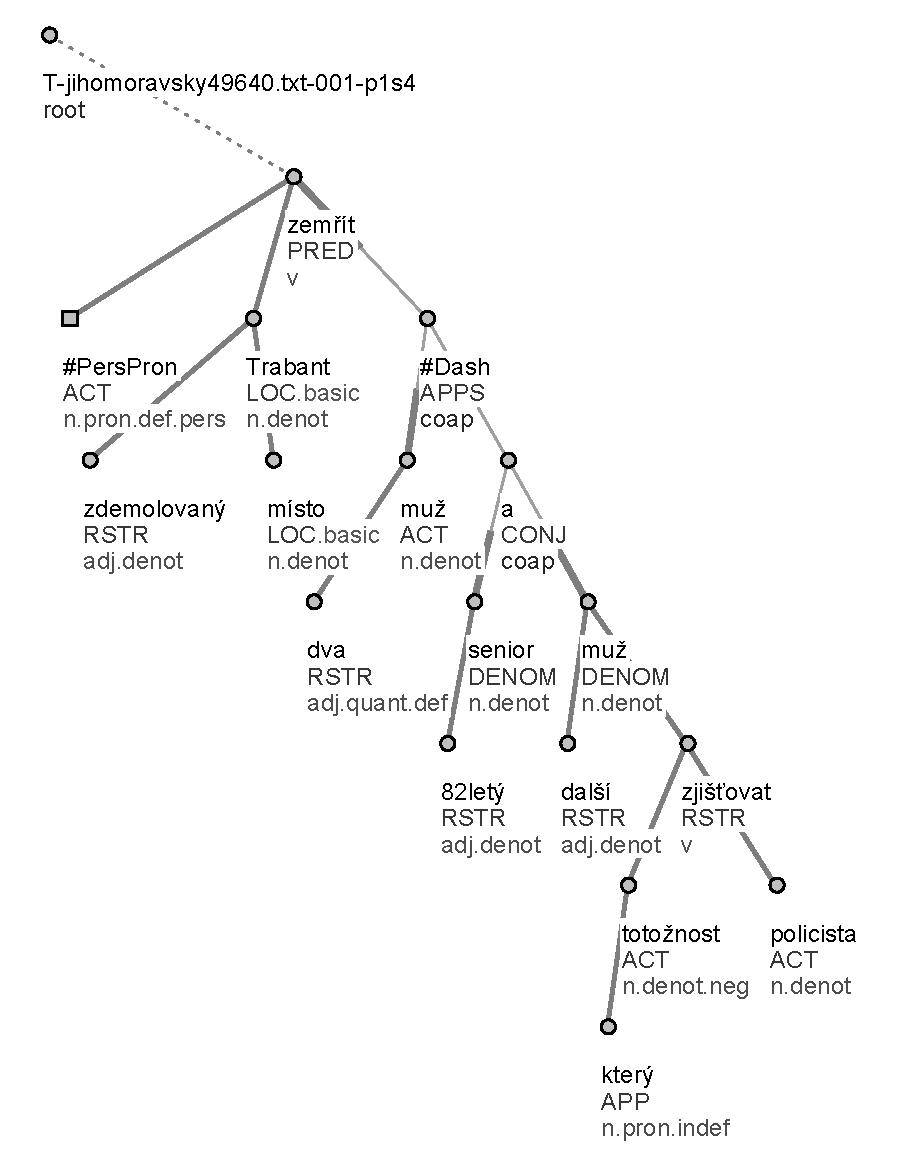
\includegraphics[width=.6\hsize]{img/TectogramaticalTree}
\caption{A tectogrammatical tree of sentence: ``Two men died on the spot in the demolished Trabant...''}
\label{img:tectogrammatical}
\end{figure}



\section{Domain dependent automated annotation}
Second phase of our extraction-annotation process is domain dependent. It makes use of previous intermediate general (domain independent) annotation. Our goal is to make this process as fast and as easy as possible, e.g. to be trained very fast (possibly in query time) and precisely by any user with average computer skills.

\subsection{Extraction and annotation based on extraction ontology} \label{sec:ddstruct}
Domain ontology is the basis for extraction ontology. Extraction ontology \cite{biblio:Embley02automaticallyextracting} extends the domain ontology by adding some additional information about how the instances of a class are presented on web pages. We used regular expressions to determine values of the properties. These regular expressions are matched against relevant pieces of text found on the web page in previous general annotation phase. These regular expressions are not dependent on an extraction tool, so the extraction ontology is general -- it contains generally applicable information, which can be shared and imported to the particular tool from variety of locations.

So far the creation of extraction ontology has to be done by a very experienced user and has to be verified on a set of web pages. In the future we plan to invest more effort and soft computing techniques in automating this part. In this paper we do not deal with learning of extraction ontology. 

%Please notice, that parts of domain ontology are properties \emph{ratioOfAccidents} and \emph{ratioOfDeath}, which have cumulative values obtained from linguistic extraction over the whole corpus. 
 
\subsection{Domain dependent annotation based on linguistics}

Assume we have pages annotated by a linguistic annotator and we have a domain ontology. The extraction method we have used is based on extraction rules. An example of such an extraction rule is on Figure \ref{img:ExtractionOntology} (on the left side). These rules represent common structural patterns that occur in sentences (more precisely in corresponding trees) with the same or similar meaning. Mapping of the extraction rules to the concepts of the target ontology enables the semantic extraction. Example of such a mapping is demonstrated in Figure \ref{img:ExtractionOntology}. This method is not limited to Czech language and can be used with any structured linguistic representation. We have published this method in \cite{biblio:DeVoComputingaggregations2008}, you con find more details there.


\begin{figure}
\centering
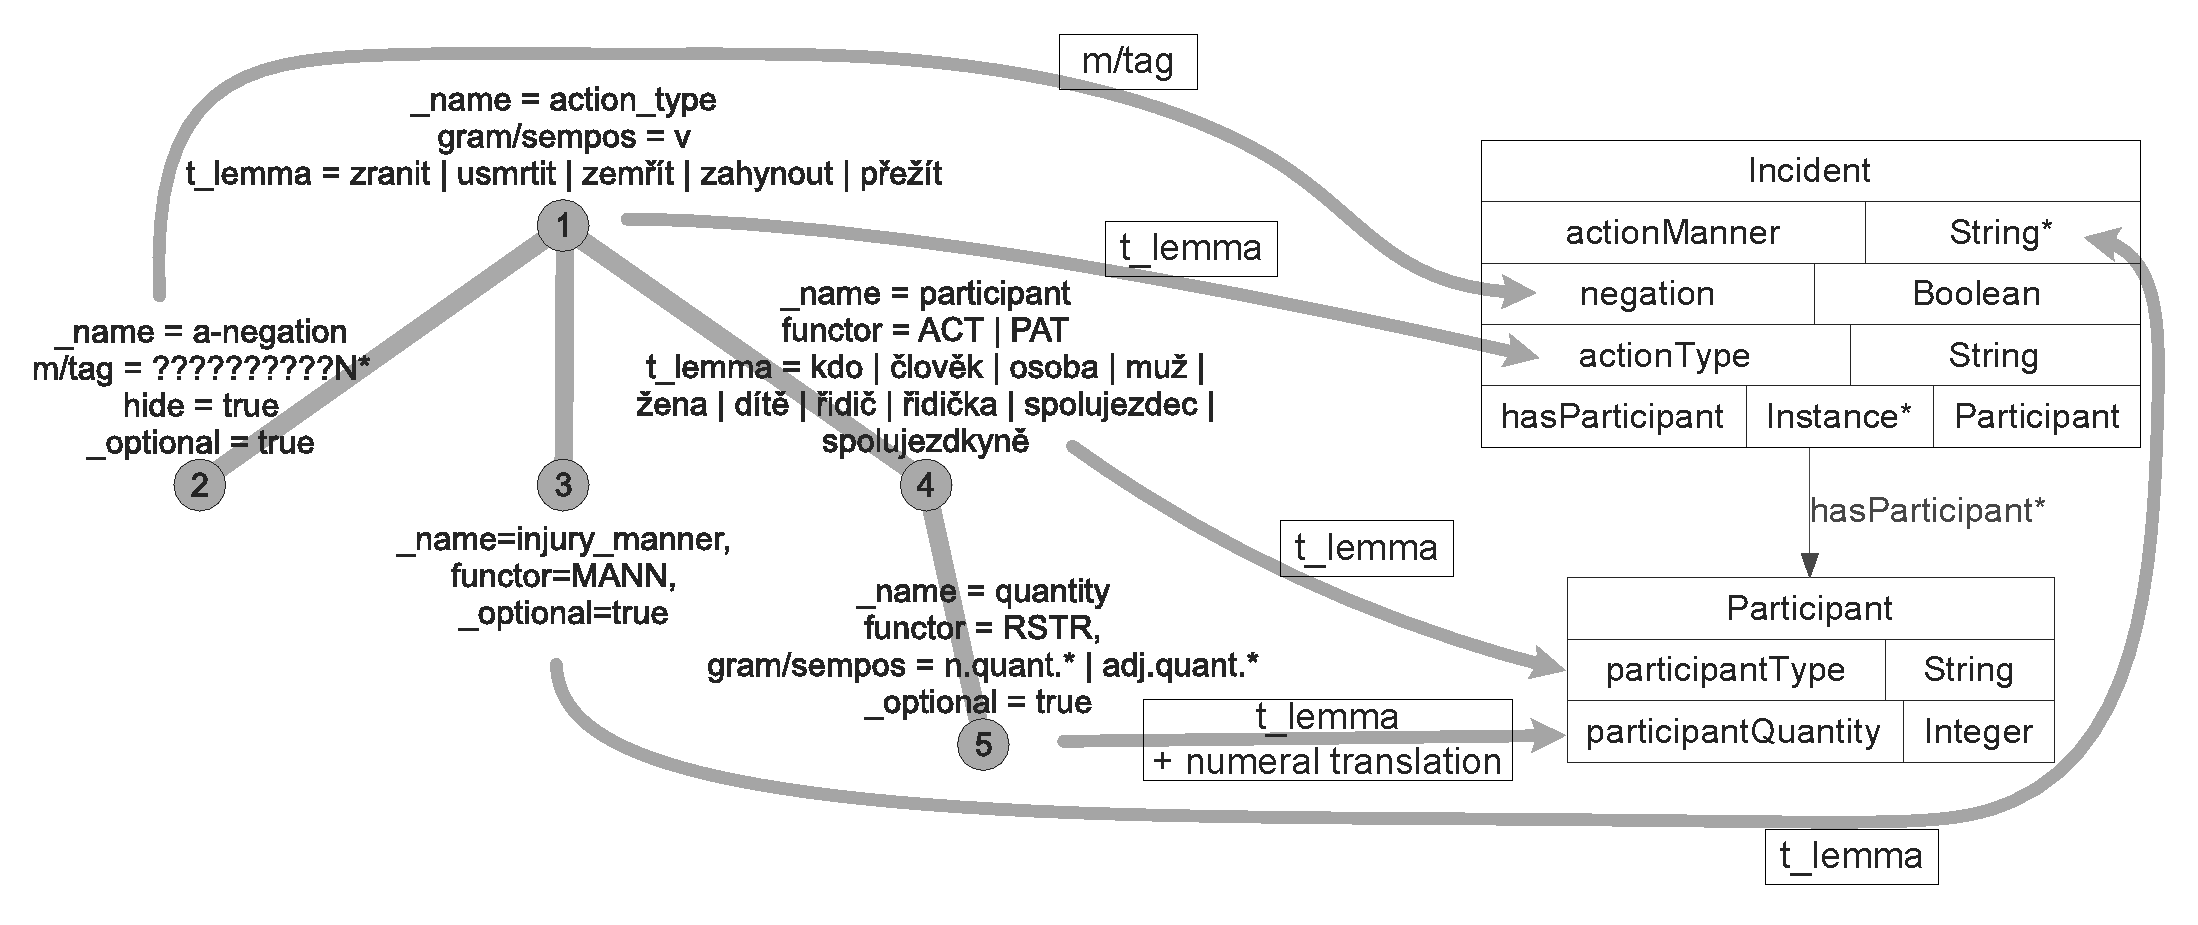
\includegraphics[width=\hsize]{img/ExtractionOntology}
\caption{An example of extraction rule and its mapping to ontology}
\label{img:ExtractionOntology}
\end{figure}

We experimented with obtaining extraction rules in two ways.
\begin{enumerate}
\item Rules and mappings were designed manually (like the rule on the Fig. \ref{img:ExtractionOntology}). 
\item Rules and mappings were learned using Inductive Logic Programming (ILP) methods (see following section).
\end{enumerate}
 Finally, having this mapping, we can extract instances of the target ontology from the answer corresponding to an extraction rule. This answer is given by the semantic repository, and the instances of the ontology are also stored there.

\subsection{Using Inductive Logic Programming (ILP)}
ILP \cite{biblio:Muggleton} is a method for a generation of rules that describe some properties of data. ILP takes three kinds of input
\begin{itemize}
	\item Positive examples E+ -- objects that have the desired property.
	\item Negative examples E- -- objects that do not have the desired property.
	\item Background knowledge -- facts about the domain (so far we do not consider background knowledge in the form of rules).
\end{itemize}

\begin{figure}
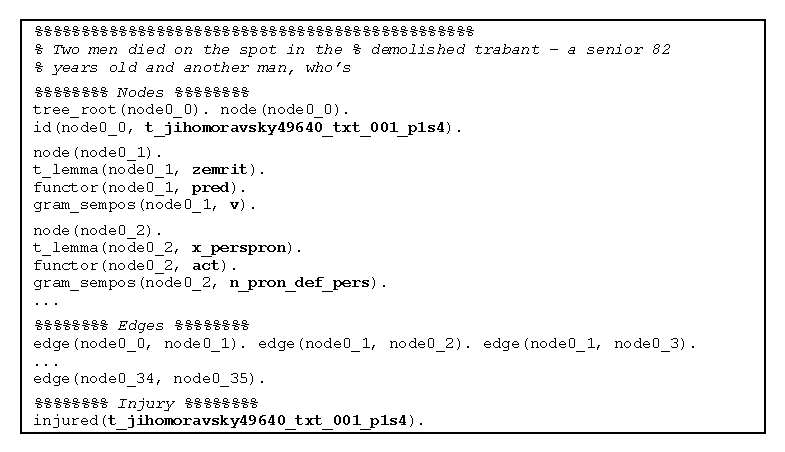
\includegraphics[width=\hsize]{img/DedEckVoj_Prolog}
\caption{Sample from prolog representation of a sentence }
\label{img:prologFacts}
\end{figure}

ILP tries to generate such rules that all positive examples and no negative example satisfy them. It uses concepts from the background knowledge in the body of the rules.
The main advantage of ILP is that it can be trained to mine arbitrary data described in predicate logic - the process of learning is dependent only on the positive and the negative examples and on the amount of information we have about them. The more information we have, the more precise the learning will be. \par

Thanks to the fact that ILP learns from positive and negative examples, we can propose an assisted learning procedure for learning and also tuning the extractor (described in previous section). The process is such that the extractor gets pure textual or semantically annotated (by the linguistic extractor) data from a web page and presents it to the user. He or she then annotates the data or only corrects the data saying which are well and which are badly annotated. The extractor can be taught and tuned to the desired goal in this way. Of course the user has to understand the semantics of the annotations - so he or she has to be an expert in that way of understanding the target ontology. Yet this ontology can be quite simple in the case we are interested only in a specific kind of information e.g. number of people injured during a car accident like in our experiments (see next section) and motivation. 

We discovered that we can use a straightforward transformation of linguistic trees (see an example on the Figure \ref{img:tectogrammatical}) to predicates of ILP (example of the transformation is in the Figure \ref{img:prologFacts}) and the learning procedure responds with significant results, which are presented in next section.

On the Figure \ref{img:tectogrammatical} we can see the relationship between particular words of a sentence and nodes of tectogrammatical tree - the highlighted node of the tree corresponds with the word `two' in the sentence (also highlighted). This relationship allows propagation of information from the user (which annotates just the text of sentence) to the ILP learning procedure.

\section{Experiments}
Our experiment was to enable our agent to access semantic information from the web. We tried to gather information form car offers with information about car accidents. We wanted to find out the number of injured persons during car accidents and match them to the offers according the car make and model. We have used firemen reports; some of them were about car accidents, some were not. Each report was split into sentences and each sentence was linguistically analyzed and transformed into a tectogrammatical tree, as described above. These trees were transformed to a set of Prolog facts (see Figure \ref{img:prologFacts}). \par
Sentences, which talk about an injury during a car accident, were manually tagged by predicate \verb#injured(X)#, where X is the ID of the sentence. Those sentences that do not talk about injured persons during a car accident were tagged as \verb#:-injured(X)#, which represents a negative example. This tagging can be done even by a user unexperienced in linguistics and ILP, but he or she has to understand the semantics of information he is tagging (in usually means that he or she has to understand the target ontology).
These tagged sentences were the input for ILP, we have used 22 sentences as positive examples and 13 sentences as negative examples.
We used Progol \cite{biblio:Muggleton2} as ILP software.
The rules ILP found are in following Figure \ref{img:rules}.

\begin{figure}
{\footnotesize
\begin{verbatim}
injured(A) :- id(B,A), id(B,t_57770_txt_001_p5s2).
injured(A) :- id(B,A), id(B,t_60375_txt_001_p1s6).
injured(A) :- id(B,A), id(B,t_57870_txt_001_p8s2).
injured(A) :- id(B,A), id(B,t_57870_txt_001_p1s1).

injured(A) :- id(B,A), edge(B,C), edge(C,D), t_lemma(D,zranit).         
injured(A) :- id(B,A), edge(B,C), edge(C,D), t_lemma(D,nehoda).
\end{verbatim}}
\caption{Rules mined by ILP}\label{img:rules}
\end{figure}

In this case we learned a set of rules that identifies relevant sentences -- roots of relevant tectogrammatical trees. We have made some additional experiments (some of them were published in \cite{biblio:DeEcExperimentswith2008}) that seems to lead to our goal. It is still a long way to go, but we understand these results as a proof of concept that ILP can be used for finding different kinds of information present in nodes and structure of linguistic trees. We for example extracted number of injured people from relevant trees when we have modified the training data. And still there is the possibility to design extraction rule manually if the learning method fails.

\section{Conclusions and further work}
In this paper we have developed the idea of web semantization, which can help to arch over the gap between Web of today and Semantic Web. We have presented a proof of concept that even today it is possible to develop a semantic search engine designed for software agents. 

%ACKNOWLEDGMENTS are optional
\subsection{Acknowledgments}
This work was partially supported by Czech projects IS-1ET100300517, GACR-201/09/H057 and MSM-0021620838.


\bibliographystyle{splncs}
\bibliography{DedekVojtas_SUM2009}  % sigproc.bib is the name of the Bibliography in this case

\end{document}
